\documentclass[twoside]{book}

% Packages required by doxygen
\usepackage{calc}
\usepackage{doxygen}
\usepackage{graphicx}
\usepackage[utf8]{inputenc}
\usepackage{makeidx}
\usepackage{multicol}
\usepackage{multirow}
\usepackage{textcomp}
\usepackage[table]{xcolor}

% Font selection
\usepackage[T1]{fontenc}
\usepackage{mathptmx}
\usepackage[scaled=.90]{helvet}
\usepackage{courier}
\usepackage{amssymb}
\usepackage{sectsty}
\renewcommand{\familydefault}{\sfdefault}
\allsectionsfont{%
  \fontseries{bc}\selectfont%
  \color{darkgray}%
}
\renewcommand{\DoxyLabelFont}{%
  \fontseries{bc}\selectfont%
  \color{darkgray}%
}

% Page & text layout
\usepackage{geometry}
\geometry{%
  a4paper,%
  top=2.5cm,%
  bottom=2.5cm,%
  left=2.5cm,%
  right=2.5cm%
}
\tolerance=750
\hfuzz=15pt
\hbadness=750
\setlength{\emergencystretch}{15pt}
\setlength{\parindent}{0cm}
\setlength{\parskip}{0.2cm}
\makeatletter
\renewcommand{\paragraph}{%
  \@startsection{paragraph}{4}{0ex}{-1.0ex}{1.0ex}{%
    \normalfont\normalsize\bfseries\SS@parafont%
  }%
}
\renewcommand{\subparagraph}{%
  \@startsection{subparagraph}{5}{0ex}{-1.0ex}{1.0ex}{%
    \normalfont\normalsize\bfseries\SS@subparafont%
  }%
}
\makeatother

% Headers & footers
\usepackage{fancyhdr}
\pagestyle{fancyplain}
\fancyhead[LE]{\fancyplain{}{\bfseries\thepage}}
\fancyhead[CE]{\fancyplain{}{}}
\fancyhead[RE]{\fancyplain{}{\bfseries\leftmark}}
\fancyhead[LO]{\fancyplain{}{\bfseries\rightmark}}
\fancyhead[CO]{\fancyplain{}{}}
\fancyhead[RO]{\fancyplain{}{\bfseries\thepage}}
\fancyfoot[LE]{\fancyplain{}{}}
\fancyfoot[CE]{\fancyplain{}{}}
\fancyfoot[RE]{\fancyplain{}{\bfseries\scriptsize Generated on Wed Nov 9 2022 15\-:49\-:12 for Project 3 by Doxygen }}
\fancyfoot[LO]{\fancyplain{}{\bfseries\scriptsize Generated on Wed Nov 9 2022 15\-:49\-:12 for Project 3 by Doxygen }}
\fancyfoot[CO]{\fancyplain{}{}}
\fancyfoot[RO]{\fancyplain{}{}}
\renewcommand{\footrulewidth}{0.4pt}
\renewcommand{\chaptermark}[1]{%
  \markboth{#1}{}%
}
\renewcommand{\sectionmark}[1]{%
  \markright{\thesection\ #1}%
}

% Indices & bibliography
\usepackage{natbib}
\usepackage[titles]{tocloft}
\setcounter{tocdepth}{3}
\setcounter{secnumdepth}{5}
\makeindex

% Hyperlinks (required, but should be loaded last)
\usepackage{ifpdf}
\ifpdf
  \usepackage[pdftex,pagebackref=true]{hyperref}
\else
  \usepackage[ps2pdf,pagebackref=true]{hyperref}
\fi
\hypersetup{%
  colorlinks=true,%
  linkcolor=blue,%
  citecolor=blue,%
  unicode%
}

% Custom commands
\newcommand{\clearemptydoublepage}{%
  \newpage{\pagestyle{empty}\cleardoublepage}%
}


%===== C O N T E N T S =====

\begin{document}

% Titlepage & ToC
\hypersetup{pageanchor=false}
\pagenumbering{roman}
\begin{titlepage}
\vspace*{7cm}
\begin{center}%
{\Large Project 3 }\\
\vspace*{1cm}
{\large Generated by Doxygen 1.8.5}\\
\vspace*{0.5cm}
{\small Wed Nov 9 2022 15:49:12}\\
\end{center}
\end{titlepage}
\clearemptydoublepage
\tableofcontents
\clearemptydoublepage
\pagenumbering{arabic}
\hypersetup{pageanchor=true}

%--- Begin generated contents ---
\chapter{\char`\"{}\-Project 3, Polymorphism and Function Efficiency\char`\"{}}
\label{index}\hypertarget{index}{}\char`\"{}\-An introduction to polymorphism, and timing the different methods to accomplish a task to determine their speed.\char`\"{} \par
\char`\"{}\-This program is made specifically for project 3.\char`\"{} \par
\char`\"{}\-It will read in a given file, and present the user with options corresponding to the read data from the file (\-As long as they are properly formatted to be inputted as a polynomial).\char`\"{} 
\chapter{Hierarchical Index}
\section{Class Hierarchy}
This inheritance list is sorted roughly, but not completely, alphabetically\-:\begin{DoxyCompactList}
\item \contentsline{section}{Dbl\-Link$<$ elt\-Type $>$}{\pageref{classDblLink}}{}
\item \contentsline{section}{Dbl\-Link$<$ Term $>$}{\pageref{classDblLink}}{}
\item \contentsline{section}{Dbl\-Link\-Itr$<$ elt\-Type $>$}{\pageref{classDblLinkItr}}{}
\item \contentsline{section}{Node$<$ elt\-Type $>$}{\pageref{classNode}}{}
\item \contentsline{section}{Node$<$ Term $>$}{\pageref{classNode}}{}
\item \contentsline{section}{Term}{\pageref{classTerm}}{}
\item \contentsline{section}{Term\-List}{\pageref{classTermList}}{}
\begin{DoxyCompactList}
\item \contentsline{section}{Term\-Array\-List}{\pageref{classTermArrayList}}{}
\item \contentsline{section}{Term\-Dbl\-Link\-List}{\pageref{classTermDblLinkList}}{}
\item \contentsline{section}{Term\-S\-T\-L\-Obj\-List}{\pageref{classTermSTLObjList}}{}
\end{DoxyCompactList}
\end{DoxyCompactList}

\chapter{Class Index}
\section{Class List}
Here are the classes, structs, unions and interfaces with brief descriptions\-:\begin{DoxyCompactList}
\item\contentsline{section}{\hyperlink{classBinaryTree}{Binary\-Tree$<$ elt\-Type $>$} }{\pageref{classBinaryTree}}{}
\item\contentsline{section}{\hyperlink{classTerm}{Term} \\*A \hyperlink{classTerm}{Term} holds one term of a polynomial }{\pageref{classTerm}}{}
\item\contentsline{section}{\hyperlink{classTermTree}{Term\-Tree} }{\pageref{classTermTree}}{}
\item\contentsline{section}{\hyperlink{classTreeNode}{Tree\-Node$<$ elt\-Type $>$} }{\pageref{classTreeNode}}{}
\end{DoxyCompactList}

\chapter{File Index}
\section{File List}
Here is a list of all documented files with brief descriptions\-:\begin{DoxyCompactList}
\item\contentsline{section}{\hyperlink{BinarySearchTree_8cpp}{Binary\-Search\-Tree.\-cpp} \\*To implement the functions prototyped in \hyperlink{BinarySearchTree_8h}{Binary\-Search\-Tree.\-h} }{\pageref{BinarySearchTree_8cpp}}{}
\item\contentsline{section}{\hyperlink{BinarySearchTree_8h}{Binary\-Search\-Tree.\-h} \\*Holds a generalized binary tree of data }{\pageref{BinarySearchTree_8h}}{}
\item\contentsline{section}{\hyperlink{Term_8cpp}{Term.\-cpp} \\*A \hyperlink{classTerm}{Term} holds a single term of a Polynomial }{\pageref{Term_8cpp}}{}
\item\contentsline{section}{\hyperlink{Term_8h}{Term.\-h} \\*An object that can hold one term of a polynomial }{\pageref{Term_8h}}{}
\item\contentsline{section}{\hyperlink{TermTree_8h}{Term\-Tree.\-h} \\*A \hyperlink{classTerm}{Term} object to print the tree in a separate manner }{\pageref{TermTree_8h}}{}
\end{DoxyCompactList}

\chapter{Class Documentation}
\hypertarget{classDblLink}{\section{Dbl\-Link$<$ elt\-Type $>$ Class Template Reference}
\label{classDblLink}\index{Dbl\-Link$<$ elt\-Type $>$@{Dbl\-Link$<$ elt\-Type $>$}}
}


\char`\"{}\-Implementation of a doubly linked list for use in project 3, used by Dbl\-Link\-List.\-h/.\-cpp\char`\"{}  




{\ttfamily \#include $<$Dbl\-Link.\-h$>$}

\subsection*{Public Member Functions}
\begin{DoxyCompactItemize}
\item 
\hypertarget{classDblLink_aa55badb70305cb5f3666ee1a0caf51bd}{\hyperlink{classDblLink_aa55badb70305cb5f3666ee1a0caf51bd}{Dbl\-Link} ()}\label{classDblLink_aa55badb70305cb5f3666ee1a0caf51bd}

\begin{DoxyCompactList}\small\item\em \char`\"{}\-Basic constructor, initializes empty list\char`\"{} \end{DoxyCompactList}\item 
\hyperlink{classDblLink_a6ec142fb189ce28f3470662d7816323c}{Dbl\-Link} (\hyperlink{classDblLink}{Dbl\-Link} \&)
\begin{DoxyCompactList}\small\item\em \char`\"{}\-Creates a deep copy construction of the list\char`\"{} \end{DoxyCompactList}\item 
\hypertarget{classDblLink_af453e027e035c5f35f57884a119111c2}{\hyperlink{classDblLink_af453e027e035c5f35f57884a119111c2}{$\sim$\-Dbl\-Link} ()}\label{classDblLink_af453e027e035c5f35f57884a119111c2}

\begin{DoxyCompactList}\small\item\em \char`\"{}\-Basic destructor, destroys list\char`\"{} \end{DoxyCompactList}\item 
\hyperlink{classDblLink}{Dbl\-Link} \& \hyperlink{classDblLink_a4ad84478d74adf66e4e8b33a790135b8}{operator=} (const \hyperlink{classDblLink}{Dbl\-Link} \&)
\begin{DoxyCompactList}\small\item\em \char`\"{}\-Assigns the contents of one doubly linked list to another\char`\"{} \end{DoxyCompactList}\item 
bool \hyperlink{classDblLink_a6967117514e7b8372e0b83cd74db0bdc}{empty} ()
\begin{DoxyCompactList}\small\item\em \char`\"{}\-Whether or not the list is currently empty\char`\"{} \end{DoxyCompactList}\item 
bool \hyperlink{classDblLink_a04b7c312227d6eabb96cbe6db17a8645}{find} (elt\-Type)
\begin{DoxyCompactList}\small\item\em \char`\"{}\-Finds the value within the doubly linked list, and remains at that element\char`\"{} \end{DoxyCompactList}\item 
void \hyperlink{classDblLink_a1eea642e9114517a9b8976bec5108612}{insert} (elt\-Type)
\begin{DoxyCompactList}\small\item\em \char`\"{}\-Inserts the given parameter to a created node before the current value\char`\"{} \end{DoxyCompactList}\item 
void \hyperlink{classDblLink_a9dee7a88fd268b8c587a6df95b4eab03}{remove} (elt\-Type)
\begin{DoxyCompactList}\small\item\em \char`\"{}\-Searches for an element in the list, and removes it if it is found\char`\"{} \end{DoxyCompactList}\end{DoxyCompactItemize}
\subsection*{Friends}
\begin{DoxyCompactItemize}
\item 
\hypertarget{classDblLink_a15e9b1e37fae72414617320686b8b4f0}{class {\bfseries Dbl\-Link\-Itr$<$ elt\-Type $>$}}\label{classDblLink_a15e9b1e37fae72414617320686b8b4f0}

\end{DoxyCompactItemize}


\subsection{Detailed Description}
\subsubsection*{template$<$class elt\-Type$>$class Dbl\-Link$<$ elt\-Type $>$}

\char`\"{}\-Implementation of a doubly linked list for use in project 3, used by Dbl\-Link\-List.\-h/.\-cpp\char`\"{} 

\subsection{Constructor \& Destructor Documentation}
\hypertarget{classDblLink_a6ec142fb189ce28f3470662d7816323c}{\index{Dbl\-Link@{Dbl\-Link}!Dbl\-Link@{Dbl\-Link}}
\index{Dbl\-Link@{Dbl\-Link}!DblLink@{Dbl\-Link}}
\subsubsection[{Dbl\-Link}]{\setlength{\rightskip}{0pt plus 5cm}template$<$typename elt\-Type $>$ {\bf Dbl\-Link}$<$ elt\-Type $>$\-::{\bf Dbl\-Link} (
\begin{DoxyParamCaption}
\item[{{\bf Dbl\-Link}$<$ elt\-Type $>$ \&}]{cl}
\end{DoxyParamCaption}
)}}\label{classDblLink_a6ec142fb189ce28f3470662d7816323c}


\char`\"{}\-Creates a deep copy construction of the list\char`\"{} 


\begin{DoxyParams}{Parameters}
{\em Dbl\-Link\&} & \char`\"{}\-The original list for copying\char`\"{} \\
\hline
\end{DoxyParams}


\subsection{Member Function Documentation}
\hypertarget{classDblLink_a6967117514e7b8372e0b83cd74db0bdc}{\index{Dbl\-Link@{Dbl\-Link}!empty@{empty}}
\index{empty@{empty}!DblLink@{Dbl\-Link}}
\subsubsection[{empty}]{\setlength{\rightskip}{0pt plus 5cm}template$<$class elt\-Type$>$ {\bf Dbl\-Link}$<$ elt\-Type $>$\-::empty (
\begin{DoxyParamCaption}
{}
\end{DoxyParamCaption}
)}}\label{classDblLink_a6967117514e7b8372e0b83cd74db0bdc}


\char`\"{}\-Whether or not the list is currently empty\char`\"{} 

\begin{DoxyReturn}{Returns}
bool \char`\"{}\-Answers true if the list is empty, false if it is not empty\char`\"{} 
\end{DoxyReturn}
\hypertarget{classDblLink_a04b7c312227d6eabb96cbe6db17a8645}{\index{Dbl\-Link@{Dbl\-Link}!find@{find}}
\index{find@{find}!DblLink@{Dbl\-Link}}
\subsubsection[{find}]{\setlength{\rightskip}{0pt plus 5cm}template$<$class elt\-Type$>$ {\bf Dbl\-Link}$<$ elt\-Type $>$\-::find (
\begin{DoxyParamCaption}
\item[{elt\-Type}]{}
\end{DoxyParamCaption}
)}}\label{classDblLink_a04b7c312227d6eabb96cbe6db17a8645}


\char`\"{}\-Finds the value within the doubly linked list, and remains at that element\char`\"{} 


\begin{DoxyParams}{Parameters}
{\em elt\-Type} & \char`\"{}\-The element to be found\char`\"{} \\
\hline
\end{DoxyParams}
\begin{DoxyReturn}{Returns}
bool \char`\"{}\-Returns true if found, false if not found\char`\"{} 
\end{DoxyReturn}
\hypertarget{classDblLink_a1eea642e9114517a9b8976bec5108612}{\index{Dbl\-Link@{Dbl\-Link}!insert@{insert}}
\index{insert@{insert}!DblLink@{Dbl\-Link}}
\subsubsection[{insert}]{\setlength{\rightskip}{0pt plus 5cm}template$<$typename elt\-Type$>$ void {\bf Dbl\-Link}$<$ elt\-Type $>$\-::insert (
\begin{DoxyParamCaption}
\item[{elt\-Type}]{x}
\end{DoxyParamCaption}
)}}\label{classDblLink_a1eea642e9114517a9b8976bec5108612}


\char`\"{}\-Inserts the given parameter to a created node before the current value\char`\"{} 


\begin{DoxyParams}{Parameters}
{\em elt\-Type} & \char`\"{}\-The element to be inputted\char`\"{} \\
\hline
\end{DoxyParams}
\hypertarget{classDblLink_a4ad84478d74adf66e4e8b33a790135b8}{\index{Dbl\-Link@{Dbl\-Link}!operator=@{operator=}}
\index{operator=@{operator=}!DblLink@{Dbl\-Link}}
\subsubsection[{operator=}]{\setlength{\rightskip}{0pt plus 5cm}template$<$typename elt\-Type $>$ {\bf Dbl\-Link}$<$ elt\-Type $>$ \& {\bf Dbl\-Link}$<$ elt\-Type $>$\-::operator= (
\begin{DoxyParamCaption}
\item[{const {\bf Dbl\-Link}$<$ elt\-Type $>$ \&}]{cl}
\end{DoxyParamCaption}
)}}\label{classDblLink_a4ad84478d74adf66e4e8b33a790135b8}


\char`\"{}\-Assigns the contents of one doubly linked list to another\char`\"{} 


\begin{DoxyParams}{Parameters}
{\em const Dbl\-Link\&} & \char`\"{}\-The list to be assigned the information\char`\"{} \\
\hline
\end{DoxyParams}
\hypertarget{classDblLink_a9dee7a88fd268b8c587a6df95b4eab03}{\index{Dbl\-Link@{Dbl\-Link}!remove@{remove}}
\index{remove@{remove}!DblLink@{Dbl\-Link}}
\subsubsection[{remove}]{\setlength{\rightskip}{0pt plus 5cm}template$<$typename elt\-Type$>$ void {\bf Dbl\-Link}$<$ elt\-Type $>$\-::remove (
\begin{DoxyParamCaption}
\item[{elt\-Type}]{x}
\end{DoxyParamCaption}
)}}\label{classDblLink_a9dee7a88fd268b8c587a6df95b4eab03}


\char`\"{}\-Searches for an element in the list, and removes it if it is found\char`\"{} 


\begin{DoxyParams}{Parameters}
{\em elt\-Type} & \char`\"{}\-The element to be removed if found\char`\"{} \\
\hline
\end{DoxyParams}


The documentation for this class was generated from the following file\-:\begin{DoxyCompactItemize}
\item 
\hyperlink{DblLink_8h}{Dbl\-Link.\-h}\end{DoxyCompactItemize}

\hypertarget{classDblLinkItr}{\section{Dbl\-Link\-Itr$<$ elt\-Type $>$ Class Template Reference}
\label{classDblLinkItr}\index{Dbl\-Link\-Itr$<$ elt\-Type $>$@{Dbl\-Link\-Itr$<$ elt\-Type $>$}}
}
\subsection*{Public Member Functions}
\begin{DoxyCompactItemize}
\item 
\hypertarget{classDblLinkItr_a029e88245826cd3f4940e8c2ccdf1508}{{\bfseries Dbl\-Link\-Itr} (const \hyperlink{classDblLink}{Dbl\-Link}$<$ elt\-Type $>$ \&list)}\label{classDblLinkItr_a029e88245826cd3f4940e8c2ccdf1508}

\item 
\hypertarget{classDblLinkItr_a1f2303149b9a0ecc0cc94fc3669d42e6}{void {\bfseries start} ()}\label{classDblLinkItr_a1f2303149b9a0ecc0cc94fc3669d42e6}

\item 
\hypertarget{classDblLinkItr_abd8531686d0efb34dfe334070755bedd}{bool {\bfseries is\-Empty} ()}\label{classDblLinkItr_abd8531686d0efb34dfe334070755bedd}

\item 
\hypertarget{classDblLinkItr_a481fe000f5c0b9e9a90c8ec947ac2366}{bool {\bfseries is\-Last\-Node} ()}\label{classDblLinkItr_a481fe000f5c0b9e9a90c8ec947ac2366}

\item 
\hypertarget{classDblLinkItr_abd2248f781624a381dcc407af0081314}{bool {\bfseries is\-First\-Node} ()}\label{classDblLinkItr_abd2248f781624a381dcc407af0081314}

\item 
\hypertarget{classDblLinkItr_ac3e8e420c63d144a562da5dbb8da9ce0}{elt\-Type {\bfseries operator$\ast$} ()}\label{classDblLinkItr_ac3e8e420c63d144a562da5dbb8da9ce0}

\item 
\hypertarget{classDblLinkItr_a6880f6792f580bcbaa677c509bcfef8a}{void {\bfseries operator++} ()}\label{classDblLinkItr_a6880f6792f580bcbaa677c509bcfef8a}

\item 
\hypertarget{classDblLinkItr_aa3dec9a784bfee4907bc1a7a94bbf1dc}{void {\bfseries operator-\/-\/} ()}\label{classDblLinkItr_aa3dec9a784bfee4907bc1a7a94bbf1dc}

\end{DoxyCompactItemize}


The documentation for this class was generated from the following file\-:\begin{DoxyCompactItemize}
\item 
Dbl\-Link.\-h\end{DoxyCompactItemize}

\hypertarget{classNode}{\section{Node$<$ elt\-Type $>$ Class Template Reference}
\label{classNode}\index{Node$<$ elt\-Type $>$@{Node$<$ elt\-Type $>$}}
}
\subsection*{Friends}
\begin{DoxyCompactItemize}
\item 
\hypertarget{classNode_a633d28fd34fd4343a6788b6eeb70f18f}{class {\bfseries Dbl\-Link$<$ elt\-Type $>$}}\label{classNode_a633d28fd34fd4343a6788b6eeb70f18f}

\item 
\hypertarget{classNode_a15e9b1e37fae72414617320686b8b4f0}{class {\bfseries Dbl\-Link\-Itr$<$ elt\-Type $>$}}\label{classNode_a15e9b1e37fae72414617320686b8b4f0}

\end{DoxyCompactItemize}


The documentation for this class was generated from the following file\-:\begin{DoxyCompactItemize}
\item 
Dbl\-Link.\-h\end{DoxyCompactItemize}

\hypertarget{classTerm}{\section{Term Class Reference}
\label{classTerm}\index{Term@{Term}}
}


\char`\"{}\-Object that contains information for a polynomial\char`\"{}  




{\ttfamily \#include $<$Term.\-h$>$}

\subsection*{Public Member Functions}
\begin{DoxyCompactItemize}
\item 
\hyperlink{classTerm_aa72ef129269040b50836346dcae32154}{Term} (double=0, int=0)
\begin{DoxyCompactList}\small\item\em "Basic constructor for the \hyperlink{classTerm}{Term} object \end{DoxyCompactList}\item 
double \hyperlink{classTerm_a51ba0eb6ed3140d3fb2fe43cc4bdcace}{get\-Coefficient} () const 
\begin{DoxyCompactList}\small\item\em \char`\"{}\-Returns the value of the coefficient of the polynomial within the object\char`\"{} \end{DoxyCompactList}\item 
int \hyperlink{classTerm_a97ab7c2fa2a3b39939c2d9b0498276ae}{get\-Exponent} () const 
\begin{DoxyCompactList}\small\item\em \char`\"{}\-Returns the value of the exponent of the polynomial within the object\char`\"{} \end{DoxyCompactList}\item 
double \hyperlink{classTerm_ab89ea23f82711d4fc9f4608d0937ce31}{operator()} (double x) const 
\begin{DoxyCompactList}\small\item\em "Returns the value of the evaluation of the polynomial given x \end{DoxyCompactList}\item 
bool \hyperlink{classTerm_a8e563a63ca972c9d2cffacb471a611a5}{operator==} (int value)
\begin{DoxyCompactList}\small\item\em \char`\"{}\-Compares one term against a value\char`\"{} \end{DoxyCompactList}\item 
bool \hyperlink{classTerm_a22d1367b67d2c2d2762392463decde13}{operator==} (const \hyperlink{classTerm}{Term} \&right)
\begin{DoxyCompactList}\small\item\em \char`\"{}\-Compares one term against another term\char`\"{} \end{DoxyCompactList}\item 
bool \hyperlink{classTerm_ade58cd311d21215402183d2dec66b48a}{operator$<$} (\hyperlink{classTerm}{Term} \&right)
\begin{DoxyCompactList}\small\item\em \char`\"{}\-Returns the bool for the term being less than another value via their exponents\char`\"{} \end{DoxyCompactList}\item 
bool \hyperlink{classTerm_a44f5d686c50172e689cf86b2c77bbc6a}{operator$<$} (int right)
\begin{DoxyCompactList}\small\item\em \char`\"{}\-Returns the bool for the term being less than an integer via it's exponent\char`\"{} \end{DoxyCompactList}\end{DoxyCompactItemize}


\subsection{Detailed Description}
\char`\"{}\-Object that contains information for a polynomial\char`\"{} 

\subsection{Constructor \& Destructor Documentation}
\hypertarget{classTerm_aa72ef129269040b50836346dcae32154}{\index{Term@{Term}!Term@{Term}}
\index{Term@{Term}!Term@{Term}}
\subsubsection[{Term}]{\setlength{\rightskip}{0pt plus 5cm}Term\-::\-Term (
\begin{DoxyParamCaption}
\item[{double}]{coeff = {\ttfamily 0}, }
\item[{int}]{expn = {\ttfamily 0}}
\end{DoxyParamCaption}
)}}\label{classTerm_aa72ef129269040b50836346dcae32154}


"Basic constructor for the \hyperlink{classTerm}{Term} object 


\begin{DoxyParams}{Parameters}
{\em double} & \char`\"{}\-Value for the coefficient of the polynomial\char`\"{} \\
\hline
{\em int} & \char`\"{}\-Value for the exponent of the polynomial\char`\"{} \\
\hline
\end{DoxyParams}


\subsection{Member Function Documentation}
\hypertarget{classTerm_a51ba0eb6ed3140d3fb2fe43cc4bdcace}{\index{Term@{Term}!get\-Coefficient@{get\-Coefficient}}
\index{get\-Coefficient@{get\-Coefficient}!Term@{Term}}
\subsubsection[{get\-Coefficient}]{\setlength{\rightskip}{0pt plus 5cm}Term\-::get\-Coefficient (
\begin{DoxyParamCaption}
{}
\end{DoxyParamCaption}
) const}}\label{classTerm_a51ba0eb6ed3140d3fb2fe43cc4bdcace}


\char`\"{}\-Returns the value of the coefficient of the polynomial within the object\char`\"{} 

\begin{DoxyReturn}{Returns}
double \char`\"{}\-Value of the coefficient\char`\"{} 
\end{DoxyReturn}
\hypertarget{classTerm_a97ab7c2fa2a3b39939c2d9b0498276ae}{\index{Term@{Term}!get\-Exponent@{get\-Exponent}}
\index{get\-Exponent@{get\-Exponent}!Term@{Term}}
\subsubsection[{get\-Exponent}]{\setlength{\rightskip}{0pt plus 5cm}Term\-::get\-Exponent (
\begin{DoxyParamCaption}
{}
\end{DoxyParamCaption}
) const}}\label{classTerm_a97ab7c2fa2a3b39939c2d9b0498276ae}


\char`\"{}\-Returns the value of the exponent of the polynomial within the object\char`\"{} 

\begin{DoxyReturn}{Returns}
double \char`\"{}\-Value of the exponent\char`\"{} 
\end{DoxyReturn}
\hypertarget{classTerm_ab89ea23f82711d4fc9f4608d0937ce31}{\index{Term@{Term}!operator()@{operator()}}
\index{operator()@{operator()}!Term@{Term}}
\subsubsection[{operator()}]{\setlength{\rightskip}{0pt plus 5cm}double Term\-::operator() (
\begin{DoxyParamCaption}
\item[{double}]{x}
\end{DoxyParamCaption}
) const}}\label{classTerm_ab89ea23f82711d4fc9f4608d0937ce31}


"Returns the value of the evaluation of the polynomial given x 


\begin{DoxyParams}{Parameters}
{\em double x} & \char`\"{}\-The value to evaluate the polynomial with\char`\"{} \\
\hline
\end{DoxyParams}
\begin{DoxyReturn}{Returns}
double \char`\"{}\-Value of the evalutaed polynomial\char`\"{} 
\end{DoxyReturn}
\hypertarget{classTerm_ade58cd311d21215402183d2dec66b48a}{\index{Term@{Term}!operator$<$@{operator$<$}}
\index{operator$<$@{operator$<$}!Term@{Term}}
\subsubsection[{operator$<$}]{\setlength{\rightskip}{0pt plus 5cm}bool Term\-::operator$<$ (
\begin{DoxyParamCaption}
\item[{{\bf Term} \&}]{right}
\end{DoxyParamCaption}
)}}\label{classTerm_ade58cd311d21215402183d2dec66b48a}


\char`\"{}\-Returns the bool for the term being less than another value via their exponents\char`\"{} 


\begin{DoxyParams}{Parameters}
{\em Term \&right} & \char`\"{}\-The value to compare to the term\char`\"{} \\
\hline
\end{DoxyParams}
\begin{DoxyReturn}{Returns}
bool \char`\"{}\-True if the exponent of the term is less than the compared one, false if else-\/wise\char`\"{} 
\end{DoxyReturn}
\hypertarget{classTerm_a44f5d686c50172e689cf86b2c77bbc6a}{\index{Term@{Term}!operator$<$@{operator$<$}}
\index{operator$<$@{operator$<$}!Term@{Term}}
\subsubsection[{operator$<$}]{\setlength{\rightskip}{0pt plus 5cm}bool Term\-::operator$<$ (
\begin{DoxyParamCaption}
\item[{int}]{right}
\end{DoxyParamCaption}
)}}\label{classTerm_a44f5d686c50172e689cf86b2c77bbc6a}


\char`\"{}\-Returns the bool for the term being less than an integer via it's exponent\char`\"{} 


\begin{DoxyParams}{Parameters}
{\em int right} & \char`\"{}\-The value to compare the term to\char`\"{} \\
\hline
\end{DoxyParams}
\begin{DoxyReturn}{Returns}
bool \char`\"{}\-True if the term's exponent is less than the integer, false if else-\/wise\char`\"{} 
\end{DoxyReturn}
\hypertarget{classTerm_a8e563a63ca972c9d2cffacb471a611a5}{\index{Term@{Term}!operator==@{operator==}}
\index{operator==@{operator==}!Term@{Term}}
\subsubsection[{operator==}]{\setlength{\rightskip}{0pt plus 5cm}bool Term\-::operator== (
\begin{DoxyParamCaption}
\item[{int}]{value}
\end{DoxyParamCaption}
)}}\label{classTerm_a8e563a63ca972c9d2cffacb471a611a5}


\char`\"{}\-Compares one term against a value\char`\"{} 


\begin{DoxyParams}{Parameters}
{\em int value} & \char`\"{}\-The value to compare the term to\char`\"{} \\
\hline
\end{DoxyParams}
\begin{DoxyReturn}{Returns}
bool \char`\"{}\-True if the polynomials exponent is the same as the integer value, false if else-\/wise\char`\"{} 
\end{DoxyReturn}
\hypertarget{classTerm_a22d1367b67d2c2d2762392463decde13}{\index{Term@{Term}!operator==@{operator==}}
\index{operator==@{operator==}!Term@{Term}}
\subsubsection[{operator==}]{\setlength{\rightskip}{0pt plus 5cm}bool Term\-::operator== (
\begin{DoxyParamCaption}
\item[{const {\bf Term} \&}]{right}
\end{DoxyParamCaption}
)}}\label{classTerm_a22d1367b67d2c2d2762392463decde13}


\char`\"{}\-Compares one term against another term\char`\"{} 


\begin{DoxyParams}{Parameters}
{\em const Term \&right} & \char`\"{}\-The term to compare the term to\char`\"{} \\
\hline
\end{DoxyParams}
\begin{DoxyReturn}{Returns}
bool \char`\"{}\-True if the terms' exponents are the same, false if else-\/wise\char`\"{} 
\end{DoxyReturn}


The documentation for this class was generated from the following files\-:\begin{DoxyCompactItemize}
\item 
\hyperlink{Term_8h}{Term.\-h}\item 
Term.\-cpp\end{DoxyCompactItemize}

\hypertarget{classTermArrayList}{\section{Term\-Array\-List Class Reference}
\label{classTermArrayList}\index{Term\-Array\-List@{Term\-Array\-List}}
}
Inheritance diagram for Term\-Array\-List\-:\begin{figure}[H]
\begin{center}
\leavevmode
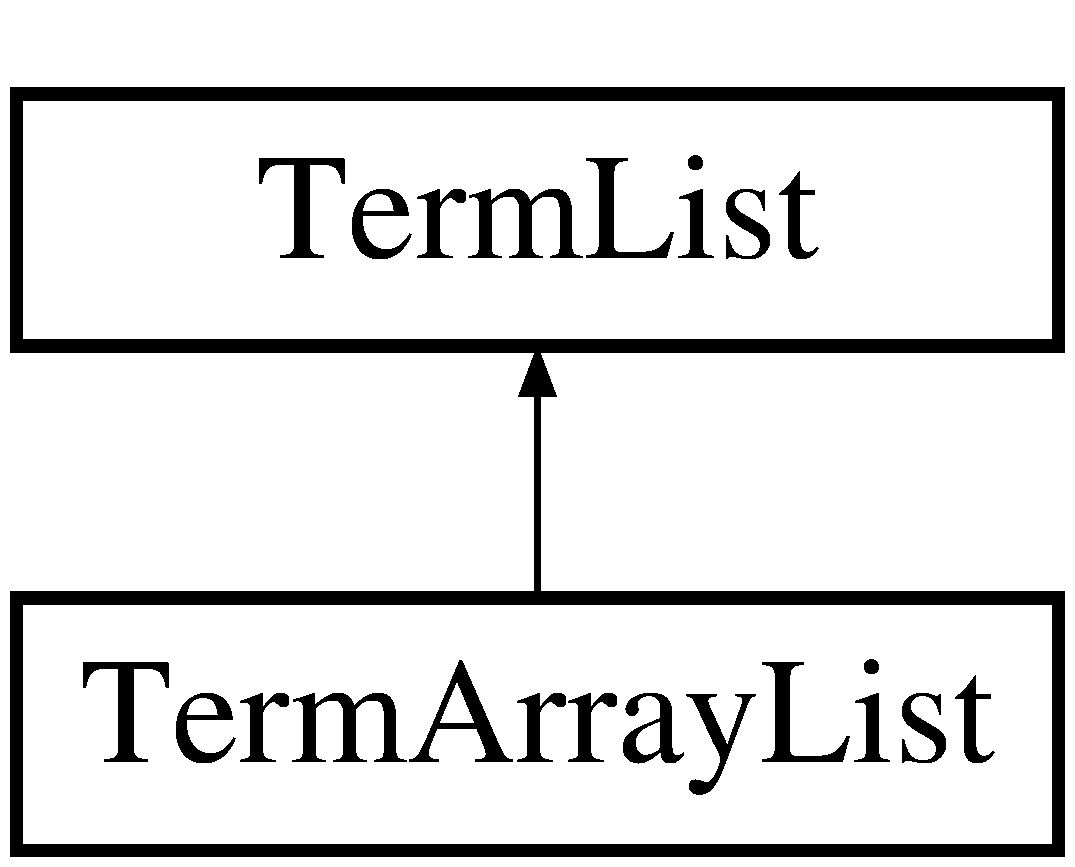
\includegraphics[height=2.000000cm]{classTermArrayList}
\end{center}
\end{figure}
\subsection*{Public Member Functions}
\begin{DoxyCompactItemize}
\item 
\hypertarget{classTermArrayList_a7abb9dc265a5d89e31bfa9caf0a0add3}{void {\bfseries read\-Into\-List} (string filename)}\label{classTermArrayList_a7abb9dc265a5d89e31bfa9caf0a0add3}

\item 
\hypertarget{classTermArrayList_a1c6a97fd1ba740bcddd6ee257ff4a088}{void {\bfseries print\-Iteratively} ()}\label{classTermArrayList_a1c6a97fd1ba740bcddd6ee257ff4a088}

\item 
\hypertarget{classTermArrayList_a6777d9358149d683902610c24c4752f6}{void {\bfseries print\-Recursively} (int x=0)}\label{classTermArrayList_a6777d9358149d683902610c24c4752f6}

\item 
\hypertarget{classTermArrayList_a0619e7312f7af5c17ef029995029fa0d}{void {\bfseries print\-Ptr} ()}\label{classTermArrayList_a0619e7312f7af5c17ef029995029fa0d}

\item 
\hypertarget{classTermArrayList_a890facace1b1acd72df0f500d9279a04}{virtual double {\bfseries operator()} (double x) const }\label{classTermArrayList_a890facace1b1acd72df0f500d9279a04}

\end{DoxyCompactItemize}


The documentation for this class was generated from the following files\-:\begin{DoxyCompactItemize}
\item 
Term\-Array\-List.\-h\item 
Term\-Array\-List.\-cpp\end{DoxyCompactItemize}

\hypertarget{classTermDblLinkList}{\section{Term\-Dbl\-Link\-List Class Reference}
\label{classTermDblLinkList}\index{Term\-Dbl\-Link\-List@{Term\-Dbl\-Link\-List}}
}
Inheritance diagram for Term\-Dbl\-Link\-List\-:\begin{figure}[H]
\begin{center}
\leavevmode
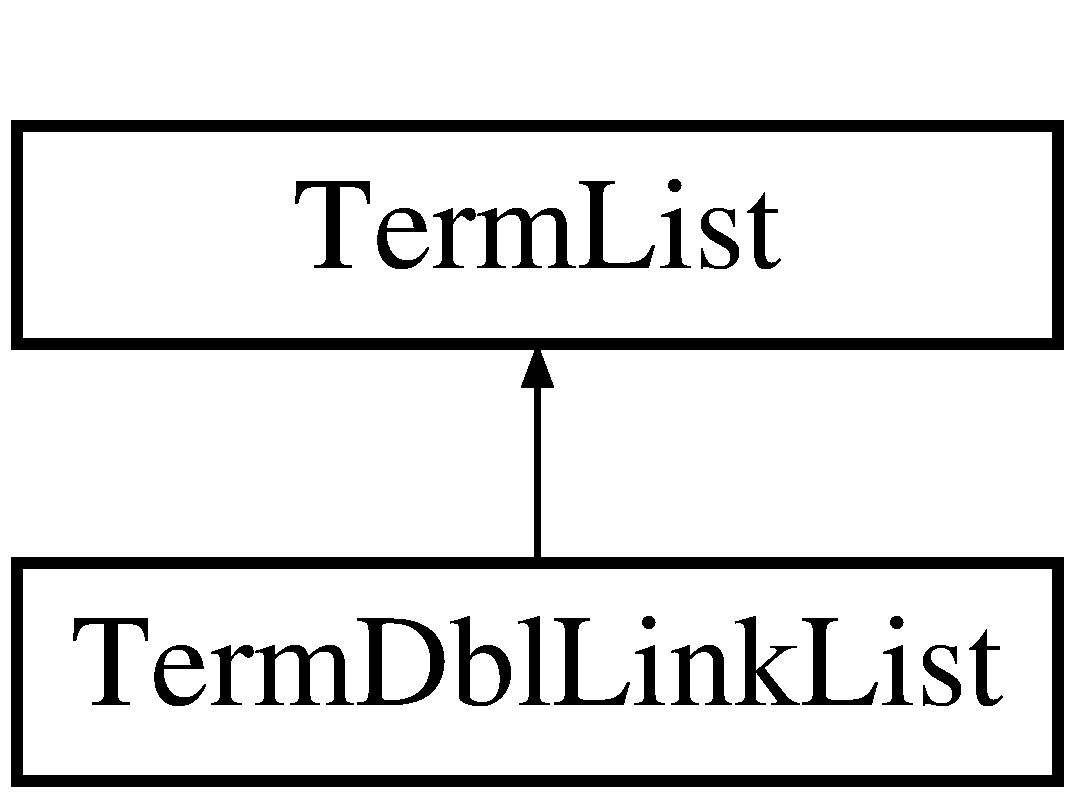
\includegraphics[height=2.000000cm]{classTermDblLinkList}
\end{center}
\end{figure}
\subsection*{Public Member Functions}
\begin{DoxyCompactItemize}
\item 
\hypertarget{classTermDblLinkList_abc5166e40aaeb0988c905cd25e1ba167}{void {\bfseries read\-Into\-List} (string filename)}\label{classTermDblLinkList_abc5166e40aaeb0988c905cd25e1ba167}

\item 
\hypertarget{classTermDblLinkList_a6acc67af3d9536fd2c409e179bec05b3}{void {\bfseries print\-Iteratively} ()}\label{classTermDblLinkList_a6acc67af3d9536fd2c409e179bec05b3}

\item 
\hypertarget{classTermDblLinkList_aa00c9ea87584a884888839ade9a1cfef}{void {\bfseries print\-Recursively} (int x=0)}\label{classTermDblLinkList_aa00c9ea87584a884888839ade9a1cfef}

\item 
\hypertarget{classTermDblLinkList_a0fb0c30585ad15c0059f3bcb44e2fab2}{virtual double {\bfseries operator()} (double x) const }\label{classTermDblLinkList_a0fb0c30585ad15c0059f3bcb44e2fab2}

\end{DoxyCompactItemize}


The documentation for this class was generated from the following files\-:\begin{DoxyCompactItemize}
\item 
Term\-Dbl\-Link\-List.\-h\item 
Term\-Dbl\-Link\-List.\-cpp\end{DoxyCompactItemize}

\hypertarget{classTermList}{\section{Term\-List Class Reference}
\label{classTermList}\index{Term\-List@{Term\-List}}
}
Inheritance diagram for Term\-List\-:\begin{figure}[H]
\begin{center}
\leavevmode
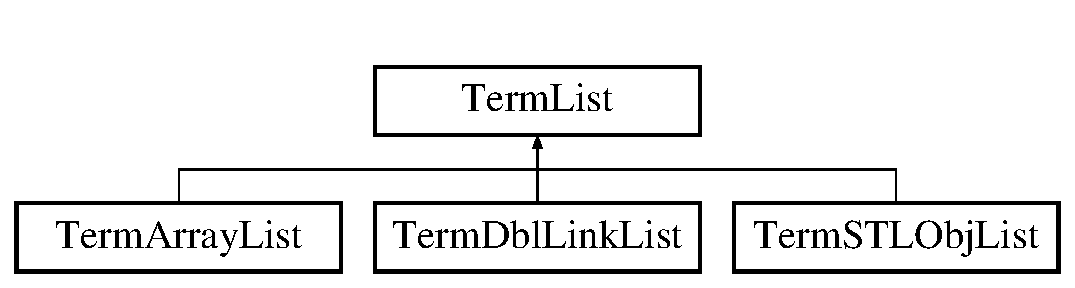
\includegraphics[height=2.000000cm]{classTermList}
\end{center}
\end{figure}
\subsection*{Public Member Functions}
\begin{DoxyCompactItemize}
\item 
\hypertarget{classTermList_a92b997bf037c009d3755440eced88b46}{virtual void {\bfseries read\-Into\-List} (string filename)=0}\label{classTermList_a92b997bf037c009d3755440eced88b46}

\item 
\hypertarget{classTermList_aecfe3d7da152b804ca9c9345d18b6909}{virtual void {\bfseries print\-Iteratively} ()=0}\label{classTermList_aecfe3d7da152b804ca9c9345d18b6909}

\item 
\hypertarget{classTermList_ae7324ddf220e93bb082dc1ac742ad698}{virtual void {\bfseries print\-Recursively} (int x=0)=0}\label{classTermList_ae7324ddf220e93bb082dc1ac742ad698}

\item 
\hypertarget{classTermList_aefbf302b65b5c423735b3a9afd7b6b62}{virtual void {\bfseries print\-Ptr} ()}\label{classTermList_aefbf302b65b5c423735b3a9afd7b6b62}

\item 
\hypertarget{classTermList_ad1600d9d577b619310f06e83e5e847ff}{virtual double {\bfseries operator()} (double x) const =0}\label{classTermList_ad1600d9d577b619310f06e83e5e847ff}

\end{DoxyCompactItemize}


The documentation for this class was generated from the following file\-:\begin{DoxyCompactItemize}
\item 
Term\-List.\-h\end{DoxyCompactItemize}

\hypertarget{classTermSTLObjList}{\section{Term\-S\-T\-L\-Obj\-List Class Reference}
\label{classTermSTLObjList}\index{Term\-S\-T\-L\-Obj\-List@{Term\-S\-T\-L\-Obj\-List}}
}


\char`\"{}\-Subclass to Term\-List, implements functions using an S\-T\-L object (\-Vector)\char`\"{}  




{\ttfamily \#include $<$Term\-S\-T\-L\-Obj\-List.\-h$>$}

Inheritance diagram for Term\-S\-T\-L\-Obj\-List\-:\begin{figure}[H]
\begin{center}
\leavevmode
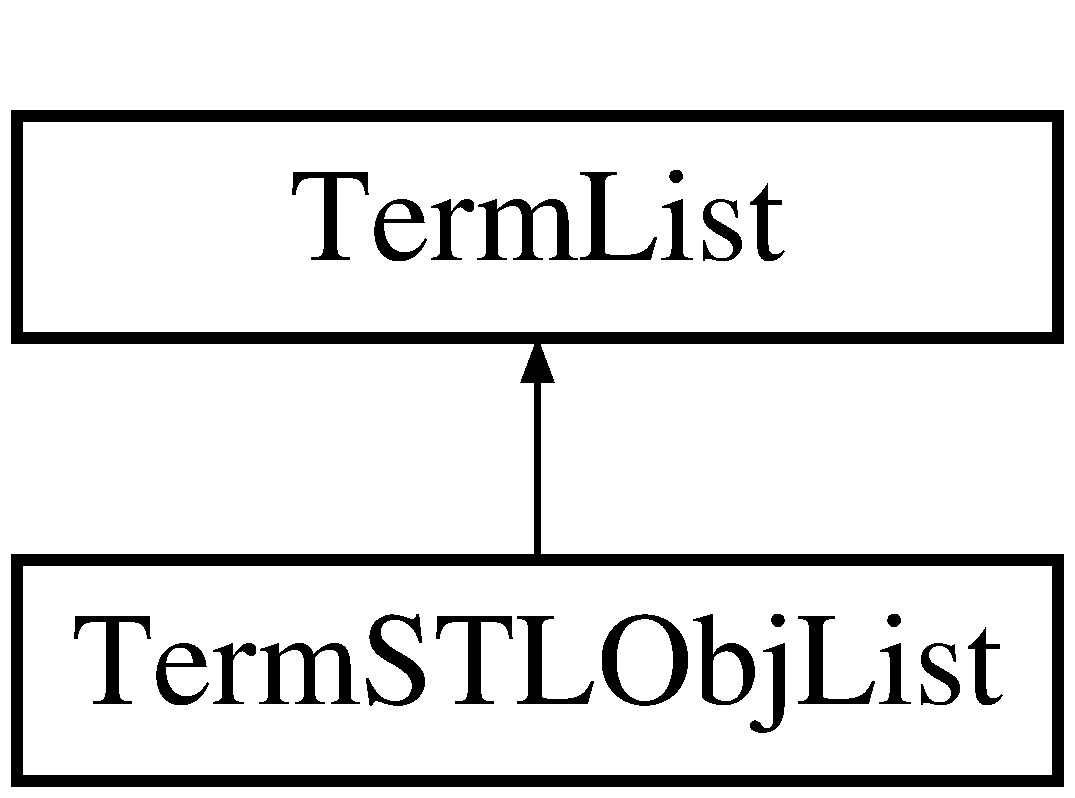
\includegraphics[height=2.000000cm]{classTermSTLObjList}
\end{center}
\end{figure}
\subsection*{Public Member Functions}
\begin{DoxyCompactItemize}
\item 
\hypertarget{classTermSTLObjList_a3dddd82683ddc17cc54e565af2ab0e0a}{\hyperlink{classTermSTLObjList_a3dddd82683ddc17cc54e565af2ab0e0a}{Term\-S\-T\-L\-Obj\-List} ()}\label{classTermSTLObjList_a3dddd82683ddc17cc54e565af2ab0e0a}

\begin{DoxyCompactList}\small\item\em \char`\"{}\-Basic constructor for Term\-S\-T\-L\-Obj\-List\char`\"{} \end{DoxyCompactList}\item 
void \hyperlink{classTermSTLObjList_a9797dc26c48d6473785d1de55b9d173f}{read\-Into\-List} (string filename)
\begin{DoxyCompactList}\small\item\em \char`\"{}\-Reads a file into the specified subclass list\char`\"{} \end{DoxyCompactList}\item 
\hypertarget{classTermSTLObjList_a4580b1ad931cb02e96485659be3e42e8}{void \hyperlink{classTermSTLObjList_a4580b1ad931cb02e96485659be3e42e8}{print\-Iteratively} ()}\label{classTermSTLObjList_a4580b1ad931cb02e96485659be3e42e8}

\begin{DoxyCompactList}\small\item\em \char`\"{}\-Prints the contents of the subclass list in an iterative method\char`\"{} \end{DoxyCompactList}\item 
void \hyperlink{classTermSTLObjList_a64b1053185cb942c6c1fa208245d1cbb}{print\-Recursively} (int x=0)
\begin{DoxyCompactList}\small\item\em \char`\"{}\-Prints the contents of the subclass list in a recursive method\char`\"{} \end{DoxyCompactList}\item 
virtual double \hyperlink{classTermSTLObjList_a72df52251f91b4ae3227af24296f0f05}{operator()} (double x) const 
\begin{DoxyCompactList}\small\item\em \char`\"{}\-Evaluates the subclass list using the value of the parameter x\char`\"{} \end{DoxyCompactList}\end{DoxyCompactItemize}


\subsection{Detailed Description}
\char`\"{}\-Subclass to Term\-List, implements functions using an S\-T\-L object (\-Vector)\char`\"{} 

\subsection{Member Function Documentation}
\hypertarget{classTermSTLObjList_a72df52251f91b4ae3227af24296f0f05}{\index{Term\-S\-T\-L\-Obj\-List@{Term\-S\-T\-L\-Obj\-List}!operator()@{operator()}}
\index{operator()@{operator()}!TermSTLObjList@{Term\-S\-T\-L\-Obj\-List}}
\subsubsection[{operator()}]{\setlength{\rightskip}{0pt plus 5cm}double Term\-S\-T\-L\-Obj\-List\-::operator() (
\begin{DoxyParamCaption}
\item[{double}]{x}
\end{DoxyParamCaption}
) const\hspace{0.3cm}{\ttfamily [virtual]}}}\label{classTermSTLObjList_a72df52251f91b4ae3227af24296f0f05}


\char`\"{}\-Evaluates the subclass list using the value of the parameter x\char`\"{} 


\begin{DoxyParams}{Parameters}
{\em double x} & \char`\"{}\-The value to be evaluated against the list\char`\"{} \\
\hline
\end{DoxyParams}


Implements \hyperlink{classTermList_ad1600d9d577b619310f06e83e5e847ff}{Term\-List}.

\hypertarget{classTermSTLObjList_a64b1053185cb942c6c1fa208245d1cbb}{\index{Term\-S\-T\-L\-Obj\-List@{Term\-S\-T\-L\-Obj\-List}!print\-Recursively@{print\-Recursively}}
\index{print\-Recursively@{print\-Recursively}!TermSTLObjList@{Term\-S\-T\-L\-Obj\-List}}
\subsubsection[{print\-Recursively}]{\setlength{\rightskip}{0pt plus 5cm}void Term\-S\-T\-L\-Obj\-List\-::print\-Recursively (
\begin{DoxyParamCaption}
\item[{int}]{x = {\ttfamily 0}}
\end{DoxyParamCaption}
)\hspace{0.3cm}{\ttfamily [virtual]}}}\label{classTermSTLObjList_a64b1053185cb942c6c1fa208245d1cbb}


\char`\"{}\-Prints the contents of the subclass list in a recursive method\char`\"{} 


\begin{DoxyParams}{Parameters}
{\em int x} & \char`\"{}\-A value to hold the recursive iteration value of the current function's phase\char`\"{} \\
\hline
\end{DoxyParams}


Implements \hyperlink{classTermList_af315579d71158e31fafa2905b20e1fa6}{Term\-List}.

\hypertarget{classTermSTLObjList_a9797dc26c48d6473785d1de55b9d173f}{\index{Term\-S\-T\-L\-Obj\-List@{Term\-S\-T\-L\-Obj\-List}!read\-Into\-List@{read\-Into\-List}}
\index{read\-Into\-List@{read\-Into\-List}!TermSTLObjList@{Term\-S\-T\-L\-Obj\-List}}
\subsubsection[{read\-Into\-List}]{\setlength{\rightskip}{0pt plus 5cm}void Term\-S\-T\-L\-Obj\-List\-::read\-Into\-List (
\begin{DoxyParamCaption}
\item[{string}]{filename}
\end{DoxyParamCaption}
)\hspace{0.3cm}{\ttfamily [virtual]}}}\label{classTermSTLObjList_a9797dc26c48d6473785d1de55b9d173f}


\char`\"{}\-Reads a file into the specified subclass list\char`\"{} 


\begin{DoxyParams}{Parameters}
{\em string filename} & \char`\"{}\-String representation of a file name, for a file to be opened and inputted into a term list\char`\"{} \\
\hline
\end{DoxyParams}


Implements \hyperlink{classTermList_a42a681a3ccc704e4a4086fcd34a01808}{Term\-List}.



The documentation for this class was generated from the following files\-:\begin{DoxyCompactItemize}
\item 
\hyperlink{TermSTLObjList_8h}{Term\-S\-T\-L\-Obj\-List.\-h}\item 
Term\-S\-T\-L\-Obj\-List.\-cpp\end{DoxyCompactItemize}

\chapter{File Documentation}
\hypertarget{app_8cpp}{\section{app.\-cpp File Reference}
\label{app_8cpp}\index{app.\-cpp@{app.\-cpp}}
}


\char`\"{}\-Driver application for project 3, 'app'\char`\"{}  


{\ttfamily \#include $<$chrono$>$}\\*
{\ttfamily \#include $<$cmath$>$}\\*
{\ttfamily \#include $<$cstdio$>$}\\*
{\ttfamily \#include $<$math.\-h$>$}\\*
{\ttfamily \#include $<$vector$>$}\\*
{\ttfamily \#include $<$iostream$>$}\\*
{\ttfamily \#include $<$fstream$>$}\\*
{\ttfamily \#include $<$iomanip$>$}\\*
{\ttfamily \#include $<$algorithm$>$}\\*
{\ttfamily \#include $<$string$>$}\\*
{\ttfamily \#include \char`\"{}Term\-List.\-h\char`\"{}}\\*
{\ttfamily \#include \char`\"{}Term\-Dbl\-Link\-List.\-h\char`\"{}}\\*
{\ttfamily \#include \char`\"{}Term\-S\-T\-L\-Obj\-List.\-h\char`\"{}}\\*
{\ttfamily \#include \char`\"{}Term\-Array\-List.\-h\char`\"{}}\\*
{\ttfamily \#include \char`\"{}Term.\-h\char`\"{}}\\*
\subsection*{Functions}
\begin{DoxyCompactItemize}
\item 
\hypertarget{app_8cpp_a695787a1e3f322fc1f5f94e9a65ef3e9}{string {\bfseries set\-File} (int argc, char $\ast$$\ast$argv)}\label{app_8cpp_a695787a1e3f322fc1f5f94e9a65ef3e9}

\item 
\hypertarget{app_8cpp_ab0d6ab2301ddc3226e50ec39805aff61}{bool {\bfseries double\-Check} (string input)}\label{app_8cpp_ab0d6ab2301ddc3226e50ec39805aff61}

\item 
\hypertarget{app_8cpp_a677fc6bddd2664cd4615201f4cb2dd23}{void {\bfseries main\-Menu} (string filename, \hyperlink{classTermList}{Term\-List} $\ast$The\-Poly, int argc, char $\ast$$\ast$argv)}\label{app_8cpp_a677fc6bddd2664cd4615201f4cb2dd23}

\item 
\hypertarget{app_8cpp_a2812aaca92daec87f2a197482eea2fac}{void {\bfseries O\-A\-Menu} (string filename, \hyperlink{classTermList}{Term\-List} $\ast$The\-Poly)}\label{app_8cpp_a2812aaca92daec87f2a197482eea2fac}

\item 
\hypertarget{app_8cpp_aa239eb6f1535b2b6288d7b71f310846e}{void {\bfseries S\-T\-Menu} (string filename, \hyperlink{classTermList}{Term\-List} $\ast$The\-Poly)}\label{app_8cpp_aa239eb6f1535b2b6288d7b71f310846e}

\item 
\hypertarget{app_8cpp_a39d82082f40bbed88fd9611b1f92fb79}{void {\bfseries D\-B\-Menu} (string filename, \hyperlink{classTermList}{Term\-List} $\ast$The\-Poly)}\label{app_8cpp_a39d82082f40bbed88fd9611b1f92fb79}

\item 
\hypertarget{app_8cpp_aaf2cebf5042a4320928335f7c90ceabf}{void {\bfseries O\-A\-It\-Print} (string filename, \hyperlink{classTermList}{Term\-List} $\ast$The\-Poly)}\label{app_8cpp_aaf2cebf5042a4320928335f7c90ceabf}

\item 
\hypertarget{app_8cpp_a169f1d1d8769856ad25895e5ec7edddc}{void {\bfseries O\-A\-Po\-Print} (string filename, \hyperlink{classTermList}{Term\-List} $\ast$The\-Poly)}\label{app_8cpp_a169f1d1d8769856ad25895e5ec7edddc}

\item 
\hypertarget{app_8cpp_ae85c32c277fe47b0983c36a346a58bce}{void {\bfseries O\-A\-Re\-Print} (string filename, \hyperlink{classTermList}{Term\-List} $\ast$The\-Poly)}\label{app_8cpp_ae85c32c277fe47b0983c36a346a58bce}

\item 
\hypertarget{app_8cpp_a7a13675ef464fbbb4cf8b4445a4a39cb}{void {\bfseries O\-A\-Poly} (string filename, \hyperlink{classTermList}{Term\-List} $\ast$The\-Poly, double x=-\/1.\-111)}\label{app_8cpp_a7a13675ef464fbbb4cf8b4445a4a39cb}

\item 
\hypertarget{app_8cpp_a01867ad0447bf9513c7b477a5fc96e9b}{void {\bfseries S\-T\-It\-Print} (string filename, \hyperlink{classTermList}{Term\-List} $\ast$The\-Poly)}\label{app_8cpp_a01867ad0447bf9513c7b477a5fc96e9b}

\item 
\hypertarget{app_8cpp_afda315a53fbfda6060f6e4124114f313}{void {\bfseries S\-T\-Re\-Print} (string filename, \hyperlink{classTermList}{Term\-List} $\ast$The\-Poly)}\label{app_8cpp_afda315a53fbfda6060f6e4124114f313}

\item 
\hypertarget{app_8cpp_a2669c4db7112ee8cd034a9f1732fe43d}{void {\bfseries S\-T\-Poly} (string filename, \hyperlink{classTermList}{Term\-List} $\ast$The\-Poly, double x=-\/1.\-111)}\label{app_8cpp_a2669c4db7112ee8cd034a9f1732fe43d}

\item 
\hypertarget{app_8cpp_a5ed338727cf32a0493d940c4f1a579ac}{void {\bfseries D\-B\-It\-Print} (string filename, \hyperlink{classTermList}{Term\-List} $\ast$The\-Poly)}\label{app_8cpp_a5ed338727cf32a0493d940c4f1a579ac}

\item 
\hypertarget{app_8cpp_ad707160a12ecc229c12a71a3573a9165}{void {\bfseries D\-B\-Re\-Print} (string filanem, \hyperlink{classTermList}{Term\-List} $\ast$The\-Poly)}\label{app_8cpp_ad707160a12ecc229c12a71a3573a9165}

\item 
\hypertarget{app_8cpp_a531a7d08da557c7bb6937f3f9c5aa00f}{void {\bfseries D\-B\-Poly} (string filename, \hyperlink{classTermList}{Term\-List} $\ast$The\-Poly, double x=-\/1.\-111)}\label{app_8cpp_a531a7d08da557c7bb6937f3f9c5aa00f}

\item 
\hypertarget{app_8cpp_a8bf194568742906b84ff2b78a2398914}{void {\bfseries O\-A\-Read} (string filename, \hyperlink{classTermList}{Term\-List} $\ast$The\-Poly)}\label{app_8cpp_a8bf194568742906b84ff2b78a2398914}

\item 
\hypertarget{app_8cpp_a174ea2318e8b9c7af4fc3e5b1ef6e055}{void {\bfseries S\-T\-Read} (string filename, \hyperlink{classTermList}{Term\-List} $\ast$The\-Poly)}\label{app_8cpp_a174ea2318e8b9c7af4fc3e5b1ef6e055}

\item 
\hypertarget{app_8cpp_a8992e01cafeb579660b8ea6c846230c5}{void {\bfseries D\-B\-Read} (string filename, \hyperlink{classTermList}{Term\-List} $\ast$The\-Poly)}\label{app_8cpp_a8992e01cafeb579660b8ea6c846230c5}

\item 
\hypertarget{app_8cpp_a3c04138a5bfe5d72780bb7e82a18e627}{int {\bfseries main} (int argc, char $\ast$$\ast$argv)}\label{app_8cpp_a3c04138a5bfe5d72780bb7e82a18e627}

\end{DoxyCompactItemize}
\subsection*{Variables}
\begin{DoxyCompactItemize}
\item 
\hypertarget{app_8cpp_a381449870b0277c80766790f99fbbacd}{ifstream {\bfseries data}}\label{app_8cpp_a381449870b0277c80766790f99fbbacd}

\end{DoxyCompactItemize}


\subsection{Detailed Description}
\char`\"{}\-Driver application for project 3, 'app'\char`\"{} 
\hypertarget{DblLink_8h}{\section{Dbl\-Link.\-h File Reference}
\label{DblLink_8h}\index{Dbl\-Link.\-h@{Dbl\-Link.\-h}}
}


\char`\"{}\-Implementation of a doubly linked list for use in project 3\char`\"{}  


{\ttfamily \#include $<$iostream$>$}\\*
\subsection*{Classes}
\begin{DoxyCompactItemize}
\item 
class \hyperlink{classDblLink}{Dbl\-Link$<$ elt\-Type $>$}
\begin{DoxyCompactList}\small\item\em \char`\"{}\-Implementation of a doubly linked list for use in project 3, used by Dbl\-Link\-List.\-h/.\-cpp\char`\"{} \end{DoxyCompactList}\item 
class \hyperlink{classDblLinkItr}{Dbl\-Link\-Itr$<$ elt\-Type $>$}
\begin{DoxyCompactList}\small\item\em \char`\"{}\-Implementation of a doubly linked list iterator for ease of use in accessing the linked list's contents\char`\"{} \end{DoxyCompactList}\item 
class \hyperlink{classNode}{Node$<$ elt\-Type $>$}
\item 
class \hyperlink{classDblLink}{Dbl\-Link$<$ elt\-Type $>$}
\begin{DoxyCompactList}\small\item\em \char`\"{}\-Implementation of a doubly linked list for use in project 3, used by Dbl\-Link\-List.\-h/.\-cpp\char`\"{} \end{DoxyCompactList}\item 
class \hyperlink{classDblLinkItr}{Dbl\-Link\-Itr$<$ elt\-Type $>$}
\begin{DoxyCompactList}\small\item\em \char`\"{}\-Implementation of a doubly linked list iterator for ease of use in accessing the linked list's contents\char`\"{} \end{DoxyCompactList}\end{DoxyCompactItemize}
\subsection*{Functions}
\begin{DoxyCompactItemize}
\item 
\hypertarget{DblLink_8h_abc7b74cba21a19ac4257e7aed66bc59e}{{\footnotesize template$<$typename elt\-Type $>$ }\\ostream \& {\bfseries operator$<$$<$} (ostream \&, \hyperlink{classDblLink}{Dbl\-Link}$<$ elt\-Type $>$)}\label{DblLink_8h_abc7b74cba21a19ac4257e7aed66bc59e}

\end{DoxyCompactItemize}


\subsection{Detailed Description}
\char`\"{}\-Implementation of a doubly linked list for use in project 3\char`\"{} 
\hypertarget{Term_8h}{\section{Term.\-h File Reference}
\label{Term_8h}\index{Term.\-h@{Term.\-h}}
}


An object that can hold one term of a polynomial.  


{\ttfamily \#include $<$iostream$>$}\\*
\subsection*{Classes}
\begin{DoxyCompactItemize}
\item 
class \hyperlink{classTerm}{Term}
\begin{DoxyCompactList}\small\item\em A \hyperlink{classTerm}{Term} holds one term of a polynomial. \end{DoxyCompactList}\end{DoxyCompactItemize}
\subsection*{Functions}
\begin{DoxyCompactItemize}
\item 
ostream \& \hyperlink{Term_8h_ad0545683062fdc76ac5b188528227353}{operator$<$$<$} (ostream \&output, const \hyperlink{classTerm}{Term} \&term)
\begin{DoxyCompactList}\small\item\em Stream insert a term. \end{DoxyCompactList}\end{DoxyCompactItemize}


\subsection{Detailed Description}
An object that can hold one term of a polynomial. 

\subsection{Function Documentation}
\hypertarget{Term_8h_ad0545683062fdc76ac5b188528227353}{\index{Term.\-h@{Term.\-h}!operator$<$$<$@{operator$<$$<$}}
\index{operator$<$$<$@{operator$<$$<$}!Term.h@{Term.\-h}}
\subsubsection[{operator$<$$<$}]{\setlength{\rightskip}{0pt plus 5cm}ostream \& operator$<$$<$ (
\begin{DoxyParamCaption}
\item[{ostream \&}]{output, }
\item[{const {\bf Term} \&}]{term}
\end{DoxyParamCaption}
)}}\label{Term_8h_ad0545683062fdc76ac5b188528227353}


Stream insert a term. 

For output 
\begin{DoxyParams}{Parameters}
{\em ofstream} & \&ouput-\/ \\
\hline
{\em const} & \hyperlink{classTerm}{Term} \&t-\/ the term object to be outputted\\
\hline
\end{DoxyParams}
\begin{DoxyReturn}{Returns}
output
\end{DoxyReturn}

\hypertarget{TermArrayList_8h}{\section{Term\-Array\-List.\-h File Reference}
\label{TermArrayList_8h}\index{Term\-Array\-List.\-h@{Term\-Array\-List.\-h}}
}


\char`\"{}\-Subclass to Term\-List, implements functions using an array\char`\"{}  


{\ttfamily \#include $<$fstream$>$}\\*
{\ttfamily \#include $<$string$>$}\\*
{\ttfamily \#include \char`\"{}Term\-List.\-h\char`\"{}}\\*
{\ttfamily \#include \char`\"{}Term.\-h\char`\"{}}\\*
\subsection*{Classes}
\begin{DoxyCompactItemize}
\item 
class \hyperlink{classTermArrayList}{Term\-Array\-List}
\begin{DoxyCompactList}\small\item\em \char`\"{}\-Subclass to Term\-List, implements functions using an array\char`\"{} \end{DoxyCompactList}\end{DoxyCompactItemize}
\subsection*{Variables}
\begin{DoxyCompactItemize}
\item 
\hypertarget{TermArrayList_8h_a4d5413895aa3b48d45f99e2ad42a4f86}{const int {\bfseries M\-A\-X\-T\-E\-R\-M\-S} =10}\label{TermArrayList_8h_a4d5413895aa3b48d45f99e2ad42a4f86}

\end{DoxyCompactItemize}


\subsection{Detailed Description}
\char`\"{}\-Subclass to Term\-List, implements functions using an array\char`\"{} 
\hypertarget{TermDblLinkList_8h}{\section{Term\-Dbl\-Link\-List.\-h File Reference}
\label{TermDblLinkList_8h}\index{Term\-Dbl\-Link\-List.\-h@{Term\-Dbl\-Link\-List.\-h}}
}


\char`\"{}\-Subclass to Term\-List, implements functions using a doubly linked list\char`\"{}  


{\ttfamily \#include $<$fstream$>$}\\*
{\ttfamily \#include $<$string$>$}\\*
{\ttfamily \#include \char`\"{}Dbl\-Link.\-h\char`\"{}}\\*
{\ttfamily \#include \char`\"{}Term\-List.\-h\char`\"{}}\\*
{\ttfamily \#include \char`\"{}Term.\-h\char`\"{}}\\*
\subsection*{Classes}
\begin{DoxyCompactItemize}
\item 
class \hyperlink{classTermDblLinkList}{Term\-Dbl\-Link\-List}
\begin{DoxyCompactList}\small\item\em \char`\"{}\-Subclass to Term\-List, implements functions using a doubly linked list\char`\"{} \end{DoxyCompactList}\end{DoxyCompactItemize}


\subsection{Detailed Description}
\char`\"{}\-Subclass to Term\-List, implements functions using a doubly linked list\char`\"{} 
\hypertarget{TermList_8h}{\section{Term\-List.\-h File Reference}
\label{TermList_8h}\index{Term\-List.\-h@{Term\-List.\-h}}
}


\char`\"{}\-Superclass to Term\-Dbl\-Link\-List, Term\-S\-T\-L\-Obj\-List, and Term\-Array\-List\char`\"{}  


{\ttfamily \#include $<$fstream$>$}\\*
{\ttfamily \#include $<$string$>$}\\*
\subsection*{Classes}
\begin{DoxyCompactItemize}
\item 
class \hyperlink{classTermList}{Term\-List}
\begin{DoxyCompactList}\small\item\em \char`\"{}\-Superclass to Term\-Dbl\-Link\-List, Term\-S\-T\-L\-Obj\-List, and Term\-Array\-List\char`\"{} \end{DoxyCompactList}\end{DoxyCompactItemize}


\subsection{Detailed Description}
\char`\"{}\-Superclass to Term\-Dbl\-Link\-List, Term\-S\-T\-L\-Obj\-List, and Term\-Array\-List\char`\"{} 
\hypertarget{TermSTLObjList_8h}{\section{Term\-S\-T\-L\-Obj\-List.\-h File Reference}
\label{TermSTLObjList_8h}\index{Term\-S\-T\-L\-Obj\-List.\-h@{Term\-S\-T\-L\-Obj\-List.\-h}}
}


\char`\"{}\-Subclass to Term\-List, implements functions using an S\-T\-L object (\-Vector)\char`\"{}  


{\ttfamily \#include $<$vector$>$}\\*
{\ttfamily \#include $<$fstream$>$}\\*
{\ttfamily \#include $<$string$>$}\\*
{\ttfamily \#include \char`\"{}Term\-List.\-h\char`\"{}}\\*
{\ttfamily \#include \char`\"{}Term.\-h\char`\"{}}\\*
\subsection*{Classes}
\begin{DoxyCompactItemize}
\item 
class \hyperlink{classTermSTLObjList}{Term\-S\-T\-L\-Obj\-List}
\begin{DoxyCompactList}\small\item\em \char`\"{}\-Subclass to Term\-List, implements functions using an S\-T\-L object (\-Vector)\char`\"{} \end{DoxyCompactList}\end{DoxyCompactItemize}


\subsection{Detailed Description}
\char`\"{}\-Subclass to Term\-List, implements functions using an S\-T\-L object (\-Vector)\char`\"{} 
%--- End generated contents ---

% Index
\newpage
\phantomsection
\addcontentsline{toc}{part}{Index}
\printindex

\end{document}
